\documentclass{article}[18pt]
\usepackage{../../../../format}
\lhead{Programming Paradigms - Functional Programming}
\usepackage{minted}
\setminted{tabsize=4}
\begin{document}
\begin{center}
\underline{\huge Recursion and higher order functions}
\end{center}
\section{Advice when writing recursive functions}
\begin{enumerate}
	\item Define the type
	\item Enumerate the cases
	\item Define simple or base cases
	\item Define the reduction of other cases to simpler ones
	\item (optional) generalise and simplify
\end{enumerate}
\section{Example: drop}
\begin{enumerate}
	\item Define the type\\
Drop the first n elements from a list:
\begin{minted}{haskell}
drop :: Int -> [a] -> [a]
\end{minted}
	\item Enumerate the cases\\
Two cases each for the integer and the list argument
\begin{minted}{haskell}
drop 0 [] =
drop 0 (x:xs) = 
drop n [] = 
drop n (x:xs) = 
\end{minted}
	\item Define simple or base cases\\
Zero and the empty list are fixed points
\begin{minted}{haskell}
drop 0 [] = []
drop 0 (x:xs) = x:xs
drop n [] = []
drop n (x:xs) = 
\end{minted}
	\item Define the reduction of other cases to simpler ones\\
Apply drop to the tail
\begin{minted}{haskell}
drop 0 [] = []
drop 0 (x:xs) = x:xs
drop n [] = []
drop n (x:xs) = drop (n-1) xs
\end{minted}
	\item (optional) generalise and simplify\\
Compress cases
\begin{minted}{haskell}
drop :: Int -> [a] -> [a]
drop 0 xs = xs
drop _ [] = []
drop n (x:xs) = drop (n-1) xs
\end{minted}
\end{enumerate}
\section{Equivalence of recursion and iteration}
\begin{itemize}
	\item Both purely iterative and purely recursive programming languages are Turing complete
	\item Hence, it is always possible to transform from one representation to the other
	\item Which is convenient depends on the algorithm, and the programming languages
\end{itemize}
Recursion $\Rightarrow$ Iteration
\begin{itemize}
	\item Write looping constructs, manually manage function call stack
\end{itemize}
Iteration $\Rightarrow$ recursion
\begin{itemize}
	\item Turn loop variables into additional function arguments
	\item And write tail recursive function (see later)
\end{itemize}
\section{How are function calls managed}
Usually a stack is used to manage nested function calls
\begin{minted}{haskell}
length' :: [a] -> Int
length' [] =0
length' (x:xs) = 1 + length' xs
\end{minted}
Calling length' on [1,2,3] does:
\begin{center}
	\includegraphics[scale=1]{"Function Calls"}
\end{center}
\begin{itemize}
	\item Each entry on the stack uses memory
	\item Too many entries cases errors: the dreaded stack overflow
	\item How big this stack is depends on the language
	\item Typically "small" in imperative languages and "big" in functional ones
\end{itemize}
\section{Typically don't have to worry about stack overflows}
\begin{itemize}
	\item In traditional imperative languages, we often try and avoid recursion
	\item Function calls are more expensive than just looping
	\item Deep recursion can result in stack overflow
	\item In contrast, Haskell is fine with much deeper recursion
	\item Unsurprising, given the programming model
	\item Still prefer to avoid recursion trees that are too deep
\end{itemize}
\section{Classifying recursive functions}
\begin{itemize}
	\item Since it is natural to write recursive functions, it makes sense to think about classifying the different types we can encounter
	\item Classifying the type of recursion is useful to allow us to think about better/cheaper implementations
\end{itemize}
Linear recursion - only contains a single self reference
\begin{minted}{haskell}
length' [] = []
length' (_:xs) = 1 + length' xs
\end{minted}
Multiple recursion - The recursive call contains multiple self references
\begin{minted}{haskell}
fib 0 = 0
fib 1 = 1
fib n = fib (n-1) + fib (n-2)
\end{minted}
Direct recursion - The function calls itself recursively
\begin{minted}{haskell}
product' [] = []
product' (x:xs) = x * product' xs
\end{minted}
Mutual/indirect recursion - multiple functions call each other recursively
\begin{minted}{haskell}
even' :: Integral a => a -> Bool
even' 0 = True
even' n = odd' (n-1)

odd' Integral a => a -> Bool
odd' 0 = False
odd' n = even' (n-1)
\end{minted}

A function is 1 of the 1st two and 1 of the 2nd two
\section{Tail recursion: a special case}
\begin{defin}[Tail recursion]
A function is tail recursive if the last result of a recursive call is the result of the function itself.\\
Loosely, the last thing a tail recursive function does is call itself with new arguments, or return a value
\end{defin}
\begin{itemize}
	\item Such functions are useful because they have a trivial translation into loops
	\item Some languages (e.g. Scheme) guarantee that a tail recursive call will be transformed into a "loop-like" implementation using a technique called tail call elimination
	\item Complexity remains unchanged, but implementation is more efficient
	\item In haskell implementations, while nice, this is not so important
\end{itemize}
\section{Iteration $\Leftrightarrow$ tail recursion}
Loops are convenient:
\begin{minted}{python}
def factorial (n):
	res = 1
	for i in range(n,1,-1)
		res *= i
	return res
\end{minted}
\textbf{Tail recursive implementation}
\begin{itemize}
	\item We can't write this directly, since we're not allowed to mutate things
	\item We can write it with a helper recursive function where all loop variables become arguments to the function
\end{itemize}
\begin{minted}{haskell}
factorial n = loop n 1
	where loop n res | n<0	   = undefined
					 | n>1	   = loop (n-1)(res*n)
					 | otherwise = res
\end{minted}
\section{What about complexity?}
\begin{itemize}
	\item Linear recursion often appears in list traversals. Typically make $\mathcal{O}(n)$ recursive calls on data of size n
	\item Multiple recursion often appears in tree or graph traversals, as well as "divide and conquer" algorithms. Number of recursive calls more problem dependent
\end{itemize}
\section{Maps and folds}
\subsection{Higher order functions}
We've seen many functions that are naturally recursive\\
We'll now look at higher order functions in the standard library that capture many of these patterns
\begin{defin}[Higher order function]
A function that does at least one of:
\begin{itemize}
	\item Take one or more functions as arguments
	\item Returns a function as its result
\end{itemize}
\end{defin}
Due to currying, every function of more than one argument is higher order in haskell
\subsubsection{Why are they useful?}
\begin{itemize}
	\item Common programming idioms can be written as functions in the language
	\item Domain specific languages can be defined with appropriate collections of higher order functions
	\item We can use the algebraic properties of higher order functions to reason about programs $\Rightarrow$ provably correct program transformations
	\item [$\Rightarrow$] Useful for domain specific compilers and automated program generation
\end{itemize}
\subsubsection{Higher order functions on lists}
\begin{itemize}
	\item Many linear recursive functions on lists can be written using higher order library functions.
	\item map: apply a function to a list
\begin{minted}{haskell}
map :: (a -> b) -> [a] -> [b]
map _ [] = []
map f xs [f x | x <- xs]
\end{minted}
	\item filter: remove entries from a list
\begin{minted}{haskell}
filter :: (a -> Bool) -> [a] -> [a]
filter _ [] = []
filter p xs = [x | x <- xs, p x]
\end{minted}
\end{itemize}
\subsection{Function composition}
\begin{itemize}
	\item Often tedious to write brackets and explicit variable names
	\item Can use function composition to simplify this
$$(f \circ g)(x) = f(g(x))$$
	\item Haskell uses the (.) operator
\begin{minted}{haskell}
(.) :: (b -> c) -> (a -> b) -> (a -> c)
f . g = \backslash x -> f (g (x))
-- example
odd a = not (even a)
odd   = not . even -- no need for the variable
\end{minted}
	\item Useful for writing compositions of functions to be passed to other higher order functions
	\item Removes need to write $\lambda$-expressions
\end{itemize}
\subsection{Folds}
\begin{itemize}
	\item Folds process a data structure in some order and build a return value
	\item Haskell provides a number of these in the standard prelude, with more available in the \texttt{Data.List} module
\end{itemize}
\subsubsection{foldr: right associative fold}
Process list from the front
\begin{minted}{haskell}
foldr :: (a -> b -> b) -> b -> [a] -> b
foldr f z []     = z
foldr f z (x:xs) = x `f` (foldr f z xs)
\end{minted}
\begin{center}
	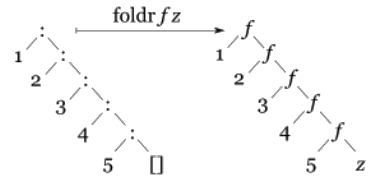
\includegraphics[scale=0.8]{foldr}
\end{center}
\subsubsection{foldl: left associative fold}
Processes list from the back (implicitly in reverse)
\begin{minted}{haskell}
foldl :: (b -> a -> b) -> b -> [a] -> b
foldl f z []     = z
foldl f z (x:xs) = foldl f (z `f` x) xs -- tail recursive
\end{minted}
\begin{center}
	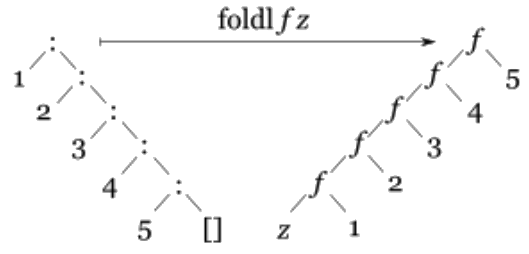
\includegraphics[scale=0.6]{foldl}
\end{center}
\subsubsection{Why would I use them?}
\begin{itemize}
	\item Capture many linear recursive patterns cleanly
	\item Can have efficient library implementation $\Rightarrow$ can apply program optimisations
	\item Actually apply to all \mintinline{haskell}{Foldable} types, not just lists
	\item e.g. \mintinline{haskell}{foldr}'s type is actually
\begin{minted}{haskell}
foldr :: Foldable t => (a -> b -> b) -> b -> t a -> b
\end{minted}
	\item So we can write code for lists and (say) trees identically
\end{itemize}
Folds are general:
\begin{itemize}
	\item Many library functions on lists are written using folds
\begin{minted}{haskell}
product = foldr (*) 1
sum = foldr (+) 0
maximum = foldr1 max -- foldr1 assumes list has at least one value
\end{minted}
\end{itemize}
\subsubsection{Which to choose?}
foldr:
\begin{itemize}
	\item Generally the right choice
	\item Works even for infinite lists
	\item Note \mintinline{haskell}{foldr (:) [] = id}
	\item Can terminate early
\end{itemize}
foldl:
\begin{itemize}
	\item Usually best to use strict versions
\begin{minted}{haskell}
import Data.List
foldl' -- note trailing
\end{minted}
	\item Doesn't work on infinite lists (needs start at the end)
	\item Can't terminate early
\end{itemize}
\end{document}